\section{Network Architecture}
In this section we design the architecture of our \gls{nn}. In section \ref{sec:related_work}, we explored \gls{nn} models that have applications in anomaly detection, as well as some related work that utilize these models for anomaly detection. Based on the findings in that section, we decide to base our \gls{nn} on the findings of \cite{kdd}, and construct a \gls{vae} with \gls{rnn} layers.

\subsection{Overall Structure}
We design a model for anomaly detection on multivariate time series data. It detects anomalies at the \gls{entity_level}, which means that it does not consider each univariate time series when determining whether an input is anomalous, but rather all the time series in a union.

Our model overall consists of two parts: a training module and a prediction module. Furthermore, we carry out some preprocessing of data as well as some postprocessing of results. Figure \ref{fig:nn_struct} shows the overall structure of our model.

\begin{figure}[htbp]
    \centering
    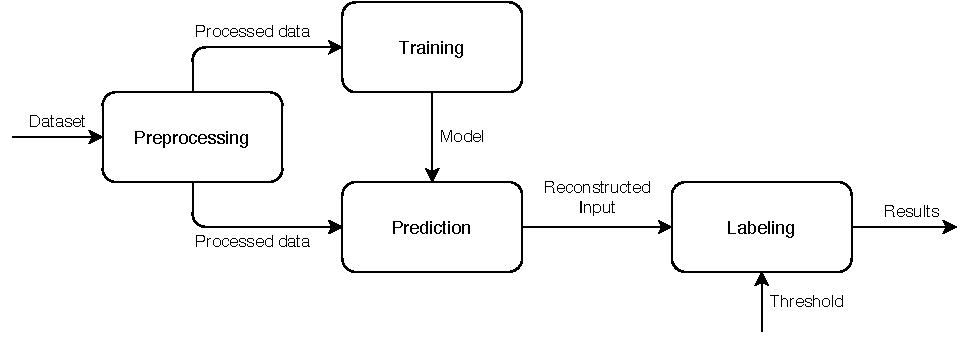
\includegraphics[width=0.9\textwidth]{Pictures/Sprint_3/NetworkStructure.pdf}
    \caption{The overall structure of our \gls{nn} model.}
    \label{fig:nn_struct}
\end{figure}
\noindent
We first perform preprocessing of the input dataset. Preprocessing is done by normalizing the input between 0 and 1, then dividing inputs into \gls{slwi} of some given size. This is done to allow the \gls{rnn} layers to capture temporal dependencies.
\\\\
The processed dataset is passed to the training module to train the model. The model is taught to reconstruct the input data as a probability distribution, such that it captures the standard patterns present in the exact data. This will, in turn, enable us to use reconstruction probabilities to determine whether a data point is anomalous.
\\\\
When the model has been trained, it may be stored and used for prediction on datasets with similar patterns. When predicting, the model will output a reconstruction of the input. This is used to compute labels for each input point.                            
\\\\
Labeling consists of computing the reconstruction probability of each input, and if that probability is lower than a threshold, the model label the input as anomalous.

\subsection{Model Architecture}
As previously explained, the model is based on the \gls{vae} model, with elements of \gls{rnn} networks, more specifically we choose to use \gls{gru} as the recurrent element in our model.

The architecture is divided into 2 logical parts, the encoder network and the decoder network. These 2 parts are very similar to the encoder and decoder networks found in auto-encoders and \glspl{vae}. Figure \ref{fig:nn_arch} shows the architecture of the encoder network and decoder network, side-by-side.

\begin{figure}[htbp]
    \centering
    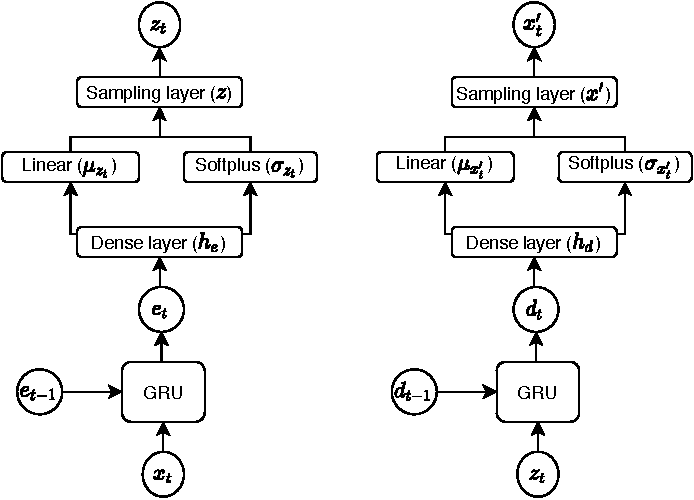
\includegraphics[width=0.8\textwidth]{Pictures/Sprint_3/NetworkArchitecture.pdf}
    \caption{Architecture of the \gls{nn}. On the left is the encoder and on the right is the decoder.}
    \label{fig:nn_arch}
\end{figure}

The encoder network consists of a \gls{gru} layer, which at time $t$ receives input $x_t$ and previous hidden state of the \gls{gru} $e_{t-1}$ to generate the hidden state $e_t$. Then $e_t$ is sent to a dense layer, $h_e$, to generate mean and standard deviation for $z_t$, $\mu_{z_t}$ and $\sigma_{z_t}$. Sampling is performed on these, as per a standard \gls{vae} through the reparameterization technique, to obtain $z_t$.

The decoder network is largely the same as the encoder network. The \gls{gru} layer receives a latent space variable at time t, $z_t$, and hidden state from previous timestep, $d_{t-1}$. The hidden state in the encoder network $e_t$ is not the same as in the decoder network $d_t$. The \gls{gru} layer then outputs hidden state $d_t$ and this is sent to the decoders dense layer, $h_d$, which in turn outputs the mean and standard deviation of $x'$, $\mu_{x'_t}$ and $\sigma_{x'_t}$.

The whole model's output is $x'_t$, which is a reconstruction of input $x$ at timestep $t$.

\subsection{Model Training}
he model can be trained by using Stochastic \gls{graddesc}.
The loss function consists of the negative reconstruction error (or negative log-likelihood) combined with the \gls{kldiv}. Thus when optimizing, we are training the network to properly reconstruct inputs based on the latent z-space variables, as well as training the network to encode inputs into a normally distributed probability distribution properly.

\subsection{Detection}
Determining whether an input $x_t$ is anomalous, the reconstruction probability of the input is calculated. The reconstruction probability of an input is a number describing how likely an input is based on the encoded latent space variable.
\\\\
Reconstruction probability $S$ is given as the following:

\begin{equation}
    S = log(p_\Theta(x_t | z_{t}))
\end{equation}

\noindent
Which is the log-probability of $x_t$ given $z_t$ and $\Theta$, where $\Theta$ are the parameters of the decoder network. If we think of the decoder network is a deterministic function that maps $z_t$ to $x'_t$, we get:

\begin{equation}
    S = log(p(x_t | x'_t))
\end{equation}

\noindent
If we assume that the $p(x_t | x'_t)$ distribution has a Gaussian form, which it should, given the applied \gls{kldiv} we get:

\begin{equation}
    S = log(p(x_t | x'_t)) \sim log e^{|x-x'|^2} \sim (x - x')^2
\end{equation}

\noindent
The decoder network is, however, not a deterministic function, but rather a stochastic function, because of the sampling layer. This means that to accurately use $(x - x')^2$, firstly, $z_t$ should be sampled many times from $\mu_{z_t}$ and $\sigma_{z_t}$, the mean of these samples calculated, and this be used as the input to the decoder network. $x'_t$ should likewise be sampled many times from $\mu_{x'_t}$ and $\sigma_{x'_t}$ and the mean should be used as $x'_t$.
\\\\
After the reconstruction probability is calculated for a single input, we need to compare it to the rest of the inputs, to determine the anomalies. This is done by computing a z-score (or standard score) for each reconstruction probability, based on all the reconstruction probabilities. The formula for calculating an inputs z-score is given as:

\begin{equation}
    \text{z-score} = \frac{x - \mu}{\sigma} 
\end{equation}

\noindent
Where $x$ is the input, $\mu$ is the mean of all the reconstruction probabilities, and $\sigma$ is the standard deviation of all the reconstruction probabilities.
\\\\
When the labeling module has calculated z-scores, it compares the scores to a threshold. A threshold is selected based on the percentile of anomalies in the input dataset. The module will label the percentile worst reconstruction probabilities as anomalies. 
For example, if a dataset is known to have $\approx 5\%$ anomalies, $\approx 2$ should be selected as a threshold, and this will mean that the $\approx 5\%$ inputs with the worst reconstruction probabilities will be labeled as anomalies.